\documentclass[../main/main.tex]{subfiles}
\begin{document}

\chapter {Physics in spacetimes}



Now that we introduced the framework of Differential Geometry, we can come back to the description of dynamics of physical systems. One one identified the metric of gravitational field, one can consider it as dynamic object. 

Before discussing the EoM of the metric we first discuss the dynamics of a (probe) particle in a fixed metric (i.e. fixed gravitational fields.
The EoM of the particle must be
\begin{enumerate}[label=(\alph*)]
\item Invariant ( in covariant form) under coordinate transformations
\item Reduce to free rectilinear motion for (flat) Minkowski metric $g=\eta$
\item Reproduce to Newton's universal law of gravitation in appropriate limit
\end{enumerate}
We will first consider (a) and (b), exploiting the \emph{least action principle}.

\section{Particle's action in flat space-time}

Let's focus to free particle in the flat space. The particle trajectories are described by world lines
\[X^\mu\,:\quad\lambda\in\RR\longmapsto X^\mu(\lambda)\in\RR^4\]
\begin{figure}[H]
\centering
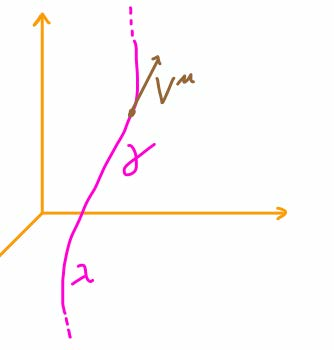
\includegraphics[width=5cm]{../img/world-line-particle-traject.jpg}
\end{figure}

In general $\lambda$ is arbitrary but if we chose it to be the proper time then the trajectory is given by a straight line, indeed for $\lambda=\tau$ and $m\neq0$
\[\alpha^\mu=0\quad\Leftrightarrow\quad\frac{\de^2 x^\mu}{\de \tau^2}=0\quad\Leftrightarrow\quad X^\mu=x_o^\mu+u^\mu\tau\]

Now we want to derive this set of equation of motions (of for each $\mu$) from a least action principle. Note that the proper time depedens on the trajectory itself, so it is not convenient to chose $\tau$ as parameter for the action. 
Since for a general $\lambda$
\begin{equation}\label{eqn:tau-lambda-relation}
\frac\de{\de\tau}=\frac{\de\lambda}{\de\tau}\frac{\de}{\de\lambda}=\frac1{\sqrt{-\eta_{\mu\nu}\dot X^\mu(\lambda)\dot X^\nu(\lambda)}}\frac\de{\de\lambda}
\end{equation}
then we can rewrite $\frac{\de^2 x^\mu}{\de \tau^2}=0$ as 
\begin{equation}
\frac{\de}{\de\lambda}\p{\frac{\eta_{\mu\nu}\dot X^\nu}{\sqrt{-\eta_{\mu\nu}\dot X^\mu\dot X^\nu}}}=0
\end{equation}
where we lowered index $\mu$ in $X\mu$ convenience. Notice that this equation is invariant under reparametrizations $\lambda\to\lambda'(\lambda)$.
Hence we want to derive this equation from least action principle. A straight world line between two points $x_{in}^\mu$ and $x_{fin}^\mu$ in $\text{Mink}_4$ is the world line that maximize the proper time $\Delta \tau$ measured along the trajectory (since along a straight world line a clock runs faster, recall twin paradox)

\begin{figure}[H]
\centering
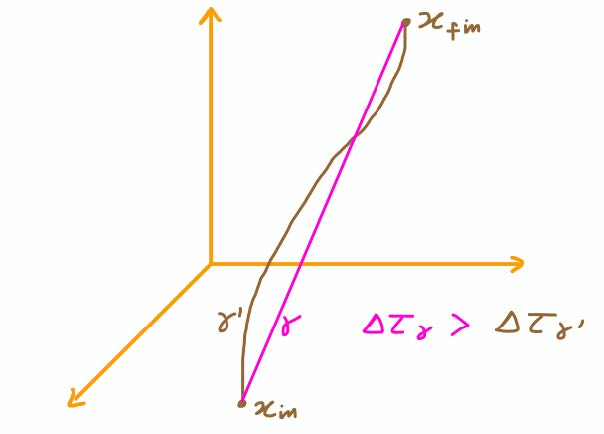
\includegraphics[width=8cm]{../img/trajectories-least-action.jpg}
\end{figure}
\noindent
This provides a natural candidate action, basically the proper time itself:
\begin{equation}\label{eqn:action-massice-part}
\boxed{
S=-m\int\de\tau=-m\int_{\lambda_{in}}^{\lambda_{fin}}\de\lambda\,\sqrt{-\eta_{\mu\nu}\dot X^\mu\dot X^\nu}
}
\end{equation}
In such a way when $\Delta \tau$ is maximum $S$ is minimum. Moreover we added the mass term $m$ in order to satisfy dimensional requirements.\footnote{In this way $[S]=EL=ET$ as we require for the action.} Notice also that this action is invariant under reparametrizations $\lambda\to\lambda'$.
If we consider a generical fluctuation $\delta X^\mu(\lambda)$ such that $\delta X^\mu(\lambda_{in})=\delta X^\mu(\lambda_{fin})=0$:
\begin{alignat*}{3}
\delta S
&=-m\int_{\lambda_{in}}^{\lambda_{fin}}\de\lambda\,\delta\sqrt{-\eta_{\mu\nu}\dot X^\mu\dot X^\nu}
&&=-m\int_{\lambda_{in}}^{\lambda_{fin}}\de\lambda\,\frac{\eta_{\mu\nu}\dot X^\mu}{\sqrt{-\eta_{\mu\nu}\dot X^\mu\dot X^\nu}}\delta\dot X^\nu\\
&=-m\int_{\lambda_{in}}^{\lambda_{fin}}\de\lambda\,\frac{\eta_{\mu\nu}\dot X^\mu}{\sqrt{-\eta_{\mu\nu}\dot X^\mu\dot X^\nu}}\frac{\de}{\de\lambda}\delta X^\nu
&&=-m\int_{\lambda_{in}}^{\lambda_{fin}}\de\lambda\,\delta X^\nu(\lambda)\frac{\de}{\de\lambda}\p{\frac{\eta_{\mu\nu}\dot X^\mu}{\sqrt{-\eta_{\mu\nu}\dot X^\mu\dot X^\nu}}}
\end{alignat*}
where in the last step we performed integration by parts with vanishing boundaries conditions. Then imposing least action principle for any fluctuation $\delta X^\nu(\lambda)$ we have
\begin{equation}
\boxed{
\delta S=0\quad\Leftrightarrow\quad\frac{\de}{\de\lambda}\p{\frac{\eta_{\mu\nu}\dot X^\mu}{\sqrt{-\eta_{\mu\nu}\dot X^\mu\dot X^\nu}}}=0
}
\end{equation}

Notice that in the massless case $m\to0$ (e.g. for photons) eq.~\eqref{eqn:action-massice-part} doesn't work, indeed we know that photons travel along null trajectories:
\[\dot X^\mu\dot X_\mu=0\quad\Rightarrow\quad \Delta\tau=0\quad\Rightarrow\quad u^\mu=\frac{\de X^\mu}{\de\tau}\text{ is not well defined}\]
However, we can avoid this problem by reformulating least action principle introducing an action that reduces to eq.~\eqref{eqn:action-massice-part} in the massive case. In order to do that, we introduce a metric on the world-line, so that the trajectory can be consider as a space-time with zero space coordinates, so that line element takes the form
\[\de s^2_\gamma=h(\lambda)\de\lambda^2=-e^2(\lambda)\de\lambda^2\]
where $h(\lambda)=g_{00}(\lambda)$ and in the second step we rewritten the line element in terms of the \emph{vielbein} one-form $e(\lambda)\de\lambda$, i.e. the basis such that the metric takes the diagonal form (for instance the basis given by eigenvectors for a matrix). In particular $[e(\lambda)\de\lambda]=\left[\frac LM\right]$ and $e(\lambda)=\tilde e(\tilde\lambda)\frac{\de\tilde\lambda}{\de\lambda}$.

Then in terms of the world line metric, or equivalently in terms of the vielbein, we can construct an alternative parametrization-invariant action
\begin{equation}\label{eqn:modif-action-flat}
\boxed{
\begin{split}
\tilde S&=-\frac12\int\de\lambda\sqrt{-h}\p{h^{-1}\dot X^\mu\dot X_\mu+m^2}\\
&=\frac12\int\de\lambda\p{e^{-1}\dot X^\mu\dot X_\mu-m^2e}
\end{split}
}
\end{equation}
In such action independent fields are not only $X^\mu$, but also one-dimensional components of $e^\mu$. This means that we promoted our time independent metric to a dynamical one by the introduction of the vielbein. On the other hand such dynamical metric, or equivalently the vielbein, appears only algebraically: it has no derivatives in the action, therefore if $m\neq0$ we can minimize action respect to fluctuations of $e$, obtaining an exact expression for $e$ in terms of coordinates $X^\mu$:
\begin{equation}\label{eqn:vielbein-m-neq0}
\delta e\quad\Longrightarrow\quad \delta \tilde S=\frac12\int\de\lambda\,\delta e\p{-\frac1{e^2}\dot X^\mu\dot X_\mu-m^2}\quad\Longrightarrow\quad e=\frac{-\sqrt{\dot X^\mu\dot X_\mu}}m
\end{equation}
In this case ($m\neq0$) the action $\tilde S$ reduces to eq.~\eqref{eqn:action-massice-part} :
\[\tilde S\big\vert_{e=\text{eq.~}\eqref{eqn:vielbein-m-neq0}}=-m\int\de\lambda\sqrt{-\dot X^\mu\dot X_\mu}=S\]
Therefore the modified action $\tilde S$ reduces to $S$ when $m\neq0$, and is a well defined action even for $m=0$. 

Before proving that $\tilde S$ provides the right EoM even for the massless case, notice that we can write $\tilde S$ in terms of the lagrangian $\tilde L$
\[\tilde S=\int\de\lambda\,\tilde L\]
and define the \textbf{4-momentum} $p^\mu$ as the conjugated field of $\dot X^\mu$
\begin{equation}\label{eqn:4-momentum-particle}
\boxed{
P_\mu\equiv\frac{\partial\tilde L}{\partial\dot X^\mu}=e^{-1}(\lambda)\eta_{\mu\nu}\dot X^\nu
}
\end{equation}
Notice that the appearance of the vielbein component leads to the invariance under reparametrization of the 4-momentum. If $m\neq0$ using eq.~\eqref{eqn:vielbein-m-neq0} with eq.~\eqref{eqn:tau-lambda-relation} the 4-momentum reduces to the standard definition
\[P^\mu=m{\frac{\de X^\mu}{\de\tau}}\]
Anyhow, notice that eq.~\eqref{eqn:4-momentum-particle} is well defined even for $m=0$.
Such massless limit can be taken even in $\tilde S$, obtaining the well defined action for massless particles
\begin{equation}
\boxed{
\tilde S\big\vert_{m\to0}=\frac12\int\de\lambda\,e^{-1}\dot X^\mu\dot X_\mu
}
\end{equation}
and the conditions we get by extremizing the action are
\begin{subequations}
\begin{align}
\delta e\quad&:\quad\dot X^\mu\dot X_\mu=0\\
\delta X^\mu\quad&:\quad\frac\de{\de\lambda}\p{e^{-1}\frac{\de X^\mu}{\de\lambda}}\equiv\frac{\de P^\mu}{\de\lambda}=0\qquad\Rightarrow\quad P^\mu(\lambda)\quad\text{is constant}
\end{align}
\end{subequations}
Notice that first condition describes the null condition for trajectories, while second conditions describes the conservation of momentum. Both result were expected according with SR.


\section{Particle's action in curved space-time}

Now we consider a free particle in a general spacetime, i.e. a particle that  interacts only with gravitational field. 
A particle's world line is now a curve in a more general 4 dimensional manifold $\mathcal M$
\[\gamma\,:\quad\RR\supset I\quad\longrightarrow\quad \mathcal M\]
\begin{figure}[H]
\centering
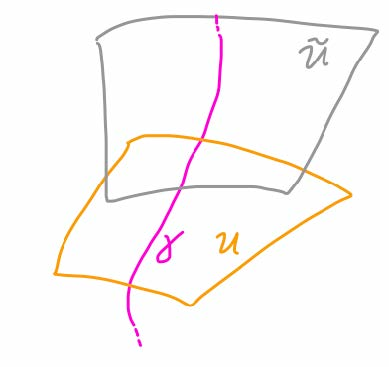
\includegraphics[width=4cm]{../img/trajectory-manifold.jpg}
\end{figure}
\noindent
In each coordinate patch $x^\mu$ the world-line is described by 4 functions
\[X^\mu\,:\quad\lambda\quad\longmapsto\quad X^\mu(\lambda)\]
In other coordinates $\tilde x^\mu=\tilde x^\mu(x)$, new coordinates are given in the intersection of opens by
\[\tilde X^\mu(\lambda)\equiv\tilde X^\mu(X(\lambda))\]

Since space-time metric can be locally well approximated by the flat one, then (smooth enough) trajectories can be locally approximated by straight world-line, tangent to $\dot X^\mu$. 

The natural requirement that no physical signal can travel faster than light translates into
\begin{equation}\label{eqn:no-faster-light-cond-metric}
g_{\mu\nu}(X)\dot X^\mu\dot X^\nu\leq0\qquad(\,<0\quad\text{for }m\neq0)
\end{equation}
\begin{figure}[H]
\centering
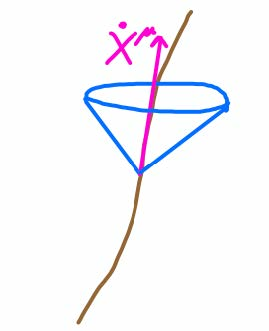
\includegraphics[width=2cm]{../img/less-than-speed-light-traj.jpg}
\end{figure}
\noindent
We can easily prove that this condition is invariant under reparametrization of $X^\mu(\lambda)$ (even for change on the direction) and also is invariant under change of patch for the manifold. 

The natural covariant generalization of eq.~\eqref{eqn:modif-action-flat} is 
\begin{equation}\label{eqn:action-curved-spacetime}
\tilde S=\frac12\int\de\lambda\p{e^{-1}g_{\mu\nu}(X)\dot X^\mu\dot X^\nu-m^2e}
\end{equation}
Notice that now also $g_{\mu\nu}(X)$ depends on $\lambda$, then  the action is not purely quadratic as in the Minkowskian case. Again, this action is invariant under transformations of $\lambda$ and $x^\mu$, in particular the invariance under changes of patch can be proven easily through transformation proprieties of tensors. 

Now we have to repeat same steps we did in the flat metric case. First let's assume $m\neq0$, then we can integrate out the world-line vielbein component as we done in eq.~\eqref{eqn:vielbein-m-neq0}:
\begin{equation}\label{eqn:vielbein-gen-m-neq0}
\delta e\quad\Longrightarrow\quad \delta \tilde S=-\frac12\int\de\lambda\,\delta e\p{\frac1{e^2}g_{\mu\nu}(X)\dot X^\mu\dot X^\nu+m^2}\quad\Longrightarrow\quad e=\frac{\sqrt{-g_{\mu\nu}\dot X^\mu\dot X^\nu}}m
\end{equation}
hence in the massive case we obtain the generalization in the curved space of the action in the massive case eq.~\eqref{eqn:action-massice-part}
\begin{equation}\label{eqn:action-massice-part-curved}
\boxed{
S=-m\int\de\lambda\sqrt{-g_{\mu\nu}\dot X^\mu\dot X^\nu}=-m\int\de\tau=-m\Delta\tau
}
\end{equation}
with:
\[\de\tau^2=-\de s^2\big\vert_\gamma=g_{\mu\nu}(X)\dot X^\mu\dot X^\nu\de\lambda^2\]
By the equivalence principle, we may again interpret $\de\tau$ and $\Delta\tau$ as proper time intervals: time intervals measured by the particle's clock. Hence, again, the particle's trajectory should be the one which (locally\footnote{For general non-trivial metrics, in particular with manifolds with non trivial topologies, may be different trajectories that maximize proper time, for instance around a cylinder one may take two paths with opposite directions that are both solutions of minimal action principle.}) maximizes the  proper time interval (between two fixed events). Notice that condition eq.\eqref{eqn:no-faster-light-cond-metric} is required in order to have a well defined squared root in eq.~\eqref{eqn:action-massice-part-curved}.

Now we have to consider the massless case, and as in the Minkowskian case we can take the massless limit directly from the action eq.~\eqref{eqn:action-curved-spacetime}:
\begin{equation}\label{eqn:action-curved-spacetime-massles}
\tilde S=\frac12\int\de\lambda\p{e^{-1}g_{\mu\nu}(X)\dot X^\mu\dot X^\nu}
\end{equation}
Taking the variation respect to the vielbein the least action principle leads to
\begin{equation}\label{eqn:action-massless-part-curved}
\delta e\quad\Longrightarrow\quad g_{\mu\nu}(X)\dot X^\mu\dot X^\nu=0
\end{equation}
hence particle moves along null trajectories. Again notice that in the massless case the vielbein is unfixed.  

The EoM for the field $X^\mu(\lambda)$ given by  action eq.~\eqref{eqn:action-curved-spacetime} are given by the least action principle respect to variation $\delta X^\mu(\lambda)$:
\begin{align*}
0=\delta\tilde S
&=\frac12\int\de\lambda\,e^{-1}\delta\p{g_{\mu\nu}(X)\dot X^\mu\dot X^\nu}\\
&=\int\de\lambda\,e^{-1}\p{g_{\mu\nu}(X)\delta\dot X^\mu\dot X^\nu+\frac12\delta X^\mu\partial_\mu g_{\nu\rho}(X)\dot X^\nu\dot X^\rho}\\
&=-\int\de\lambda\,\delta X^\mu \p{\frac\de{\de\lambda}\p{e^{-1}g_{\mu\nu}(X)\dot X^\nu}-\frac{e^{-1}}2\partial_\mu g_{\nu\rho}(X)\dot X^\nu\dot X^\rho}
\end{align*}
and we finally obtain the EoM in the curved spacetime (for both massive and massless case)
\begin{equation}
\frac\de{\de\lambda}\p{e^{-1}g_{\mu\nu}(X)\dot X^\nu}-\frac{e^{-1}}2\partial_\mu g_{\nu\rho}(X)\dot X^\nu\dot X^\rho=0
\end{equation}

Let's try to rewrite these equation of motions in a more convenient way. Remember that the vielbein transforms in a non-trivial way under reparametrizations: $\tilde e(\tilde \lambda)\frac{\de\tilde\lambda}{\de\lambda}=e(\lambda)$, then we can choose a parameter $\lambda$ such that $e(\lambda)$ is constant, just solving the first order differential equation $\tilde e(\tilde \lambda)\frac{\de\tilde\lambda}{\de\lambda}=e(\lambda)=\,$const. respect to the variable $\lambda$. Such value of $\lambda$ is said to be a \textbf{affine parameter}. For instance in the massive case $e(\lambda)=\frac1m$ corresponds to $\lambda=\tau$ (the proper time) as we can see from eq.~\eqref{eqn:vielbein-gen-m-neq0}, or, both in massive and massless case, we can always impose $e(\lambda)=1$ for some other parameter $\lambda$ (if $m\neq0$ then $\lambda=\frac\tau m$). In case $e(\lambda)=1$ we refer to the parameter $\lambda$ as \textbf{proper} parameter. 

Now, imposing $\lambda$ to be an affine parameter\footnote{This choice is said to be a \textbf{gauge choice}: we fixed a specific field $e(\lambda)$ among several equivalent choices $\tilde e(\tilde\lambda)$. This is the same we do for EM potential $A^\mu$ invariant under gauge symmetry.} the EoM can be rewritten removing the vielbein
\[
\frac\de{\de\lambda}\p{g_{\mu\nu}(X)\dot X^\nu}-\frac12\partial_\mu g_{\nu\rho}(X)\dot X^\nu\dot X^\rho=0
\]
This is consistent with the fact that EoM should not depend on the field $e(\lambda)$ we introduced in order to using Lagrangian formalism in the massless case. Writing explicitly derivatives we have
\[g_{\mu\nu}(X)\ddot X^\nu+\partial_\rho \,g_{\nu\mu}(X)\dot X^\rho\dot X^\nu-\frac12\partial_\mu g_{\nu\rho}\dot X^\nu\dot X^\rho=0\]
Notice that we may exchange indices $\rho$ and $\nu$ in the second term thanks to the symmetry of the tensor $\dot X^\mu\dot X^\nu$. Then only symmetric part of $\partial_\rho g_{\nu\mu}$ really contributes to the equation of motion
\[g_{\mu\nu}(X)\ddot X^\nu+\partial_{(\rho} \,g_{\nu)\mu}(X)\dot X^\rho\dot X^\nu-\frac12\partial_\mu g_{\nu\rho}\dot X^\nu\dot X^\rho=0\]
and taking into account this natural symmetrization we can write the EoM in the following form:
\begin{equation}\label{eqn:eom-levi-civita}
\boxed{
\frac{\de^2X^\mu}{\de\lambda^2}+\Gamma^\mu_{\nu\rho}(X)\frac{\de X^\nu}{\de\lambda}\frac{\de X^\rho}{\de\lambda}=0
}
\end{equation}
where terms
\begin{equation}\label{eqn:dfn-levi-civita-coeff}
\boxed{
\Gamma^\mu_{\nu\rho}(X)\equiv\frac12g^{\mu\sigma}(\partial_\nu g_{\rho\sigma}+\partial_\rho g_{\nu\sigma}-\partial_\sigma g_{\nu\rho})
}
\end{equation}
are known as \textbf{Christoffel symbols} or \textbf{Levi-Civita connection}.  $\Gamma^\mu_{\nu\rho}(X)$ clearly is not a tensor, anyhow its transformation proprieties must be exactly the ones of $\ddot X^\mu$ in order to satisfy eq.~\eqref{eqn:eom-levi-civita} for any choice of coordinates $X^\mu$. Moreover Christoffel symbols shows following symmetry
\[\Gamma^\mu_{\nu\rho}=\Gamma^\mu_{\rho\nu}\]

As we done for the flat space-time, we can set $\tilde S=\int\de\lambda\tilde L$ and define the four momentum in curved space as
\begin{equation}
P_\mu\equiv\frac{\partial L}{\partial \dot X^\mu}=e^{-1}\dot X^\mu\quad\rightarrow\quad P^\mu \equiv e^{-1}\dot X^\mu
\end{equation}
This formula is general for any parameter $\lambda$, but when we chose $\lambda$ to be the proper parameter ($e(\lambda)=1$) this formula reduces to 
\[P^\mu(\lambda)=\frac{\de X^\mu}{\de\lambda}\]
Recall that choice $e(\lambda)=1$ has dimension of $[\tau/m]$ i.e. a length over a mass, then $P^\mu$ has dimension of mass, which is the right dimension for the momentum when we set $c=1$.
By using this identification we can rewrite EoM in terms of 4-momentum

\begin{equation}\label{eqn:eom-levi-civita-moment}
\boxed{
\frac{\de P^\mu}{\de\lambda}+\Gamma^\mu_{\nu\rho}(X)P^\nu P^\rho=0
}
\end{equation}
This formula holds both massive and massless case, but in the massive case we have $\lambda=\frac\tau m$  and the four momentum can be written in terms of velocity:
\[P^\mu=m\frac{\de X^\mu}{\de\tau}=m u^\mu\]
then the EoM becomes
\begin{equation}\label{eqn:eom-levi-civita-velocity}
\boxed{
\frac{\de u^\mu}{\de\tau}+\Gamma^\mu_{\nu\rho}(X)u^\nu u^\rho=0
}
\end{equation}
In general (even for massless particles) $\Gamma^\mu_{\nu\rho}\neq0$ and then $P^\mu$ is not conserved:
\[\frac{\de P^\mu}{\de\lambda}=-\Gamma^\mu_{\nu\rho}(X)P^\nu P^\rho\]
In order to obtain a conserved momentum we have to require additional symmetries in our manifold, as it happen in the Minkowski case, which is the maximally symmetric space-time (since $\eta_{\mu\nu}$ is invariant under a large number of symmetries given by the Poincaré group). 
We will see that the four momentum conservation is associated to the invariance of the theory under space translations. In general only the ``lenght'' of $P^\mu$ is preserved, indeed using eq.~\eqref{eqn:action-massice-part-curved} and eq.~\eqref{eqn:action-massless-part-curved} with $e(\lambda)=1$ we obtain
\[P^\mu P_\mu=\dot X^\mu\dot X_\mu=-m^2\]
We will see in the following that eq.~\eqref{eqn:eom-levi-civita-moment} directly implies the conservation $P^\mu P_\mu$.



\section{Covariant derivatives}
\textsf{Carroll sec. 3.1,3.2}\\

Let's consider geometrical interpretation of eq.~\eqref{eqn:eom-levi-civita} and eq.~\eqref{eqn:dfn-levi-civita-coeff}  we derived in the previous lecture. All what we stated in this section hold in any metric space, not only Lorenzian ones. 

First of all notice that $\Gamma^\mu_{\nu\rho}$ soes not transform as a tensor. Rather, they define a generalization of usual derivative, the so-called \textbf{covariant derivative} $\nabla_\mu$ on vector fields, one forms, and in general on tensors
\begin{align*}
\nabla_\mu V^\mu&=\partial_\mu V^\nu+\Gamma^\nu_{\rho\mu}V^\rho\\
\nabla_\mu\alpha_\nu&=\partial_\mu\alpha_\nu-\Gamma^\rho_{\nu\mu}\alpha_\rho\\
\nabla_\mu T^{\nu\rho\dots}_{\sigma\dots}&=\partial_\mu T^{\nu\rho\dots}_{\sigma\dots}+{\Gamma^\nu}_{\tau\mu}T^{\tau\rho\dots}_{\sigma\dots}\\
&\quad+\Gamma^\rho_{\tau\mu}T^{\nu\tau\dots}_{\sigma\dots}+\dots-\Gamma^\tau_{\sigma\mu}T^{\nu\rho\dots}_{\tau\dots}-\dots
\end{align*}
Differently to usual partial derivative - which in general do not transform tensor field in tensor field - the covariant derivative $\nabla$ applied to a tensor of type $(n,m)$  produces a tensor of type $(n,m+1)$. Note that $\nabla_\mu$ preserves (anti)symmetry of indices and satisfies Leibniz rule
\[\nabla_\mu({T^\rho\dots}W_{\sigma\dots})=(\nabla_\mu T^{\rho\dots})W_{\sigma\dots}+T^{\rho\dots}\nabla_\mu W_{\sigma\dots}\]

In order to behave like a derivative (preserving tensorial nature of objects)  $\Gamma^\mu_{\nu\rho}$ must transform in such a way to ``correct'' the non-covariance of $\partial_\mu T^{\nu\dots}_{\rho\dots}$. For instance, for vector fields
\[\partial_\mu=A^\nu_\mu\tilde\partial_\nu\qquad V^\mu={(A^{-1})}^\mu_\nu\tilde V^\nu\]
with
\[\tens A\mu\nu=\pder{\tilde x^\mu}{x^\nu}\qquad\tens{(A^{-1})}\mu\nu=\pder{x^\mu}{\tilde x^\nu}\]
when we make a coordinate transformation of $\partial_\mu V^\nu$ we see that traditional derivatives do not give another vector field
\[\partial_\mu V^\nu=\tens A\rho\mu\tilde\partial_\rho(\tens{(A^{-1})}\nu\sigma\tilde V^\sigma)=\tens A\rho\mu[\tens{(A^{-1})}\nu\sigma\tilde\partial_\rho\tilde V^\sigma+(\tilde \partial_\rho\tens{(A^{-1})}\nu\tau)\tilde V^\tau]\]
I order to correct this, we have to use the covariant derivative
\begin{align*}
\nabla_\mu V^\nu
&=\partial_\mu V^\nu+\tens\Gamma\nu{\alpha\mu}V^\alpha\\
&=\tens A\rho\mu\tens{(A^{-1})}\nu\sigma[\tilde\partial_\rho\tilde V^\sigma\underbrace{\overbrace{\tens A\sigma\alpha\tilde\partial_\rho\tens{(A^{-1})}\alpha\tau}^{\tens A\sigma\alpha\tens{(A^{-1})}\beta\rho\partial_\beta\tens{(A^{-1})}\alpha\tau}\tilde V^\tau+\tens{(A^{-1})}\beta\rho\tens A\sigma\gamma\tens\Gamma\gamma{\alpha\beta}\tens{(A^{-1})}\alpha\tau\tilde V^\tau}_{\tens{\tilde\Gamma}\sigma{\tau\rho}\tilde V^\tau}]\\
&=\tens A\rho\mu\tens{(A^{-1})}\nu\sigma(\tilde\partial_\rho\tilde V^\sigma+\tens{\tilde\Gamma}\sigma{\tau\rho}\tilde V\tau)\\
&=\tens A\rho\mu\tens{(A^{-1})}\nu\sigma\tilde\nabla_\rho\tilde V^\sigma
\end{align*}
then in order to obtain a tensor as the result of the application covariant derivative to a vector field we require following transformation property under change of coordinates for Christoffel coefficients:
\begin{equation}
\tens{\tilde\Gamma}\mu{\nu\rho}=\tens A\mu\sigma\tens{(A^{-1})}\alpha\nu\tens{(A^{-1})}\beta\rho\tens\Gamma\sigma{\alpha\beta}+\tens A\mu\alpha\tens{(A^{-1})}\beta\rho\partial_\beta\tens{(A^{-1})}\alpha\nu
\end{equation}
with
\[\tens A\mu\nu=\pder{\tilde x^\nu}{x^\nu}\qquad\tens{(A^{-1})}\mu\nu=\pder{x^\mu}{\tilde x^\nu}\]
More explicitly, in coordinates
\begin{equation}\label{eqn:transf-rule-LC-coeff}\boxed{
\tchris\mu\nu\rho=\pder{\tilde x^\mu}{x^\sigma}\pder{x^\alpha}{\tilde x^\nu}\pder{x^\beta}{\tilde x\rho}\chris\sigma\alpha\beta+\pder{\tilde x^\mu}{x^\alpha}\pdder{x^\alpha}{\tilde x^\rho}{\tilde x^\nu}
}\end{equation}
This guarantees that any covariant derivative $\nabla_\mu\tens T{\rho\dots}{\nu\dots}$ transforms covariantly. One can check that Levi-Civita connection transforms according to these rules. 

Notice that
\begin{enumerate}[label=\textbullet]
\item any connection $\chris\mu\nu\rho$ must transform in this way, actually this is the defining property of a connection;
\item the non-tensorial term in eq.~\eqref{eqn:transf-rule-LC-coeff} is $\Gamma$-independent: this means that differences of connections $\Delta\chris\mu\nu\rho$ transform as tensors;
\item the antisymmetric components of coefficient of a connection\footnote{Levi-Civita coefficients are symmetric, but this does not holds in general for any connection}
\[\tens T\mu{\nu\sigma}=2\chris\mu{[\nu}{\rho]}=\chris\mu\nu\rho-\chris\mu\rho\nu\]
transforms as a tensor, and define the \textbf{torsion} tensor
\[T=2\chris\mu{[\nu}{\rho]}\partial_\mu\otimes\de x^\nu\de x^\rho\]
Clearly, for Levi-Civita connection the torsion is vanishing
\end{enumerate}

The Levi-Civita connection is the only connection that is
\begin{enumerate}
\item torsion free ($\chris\mu\nu\rho=\chris\mu\rho\nu$)
\item a metric connection such that $\nabla_\mu g_{\nu\rho}=0$, such property is called \textbf{metricity}
\end{enumerate}
One can prove that these two conditions, given some metric $g_{\mu\nu}$, define uniquely a connection, which is the Levi-Civita connection. Let's give a sketch of proof. Imposing the compatibility with the metric and the symmetry property given by $T=0$ we have
\[0=\nabla_\mu g_\nu\rho-\nabla_\nu g_{\rho\mu}-\nabla_\rho g_{\mu\nu}=\partial_\mu g_{\nu\rho}-\partial_\nu g_{\rho\mu}-\partial_\rho g_{\mu\nu}+2g_{\mu\sigma}\chris\sigma\nu\rho\]

Note that a connection $\Gamma$ is analogous to a non-abelian gauge field and indeed one can give a unified description in terms of principal and vector bundles. However, in the Standard Model the gauge fields are elementary, while in General Relativity the Levi-Civita connection $\chris\mu\nu\rho$ is composite, in terms of the elementary field $g_{\mu\nu}(x)$. 

Another important remark is that combining $g^{\mu\sigma}g_{\sigma\nu}=\delta^\mu_\nu$, $\nabla_\rho\delta_\nu^\mu=0$ (given by the fact that $\delta_\nu^\mu$ is constant) and the Leibniz rule we obtain that the covariant derivative of the inverse of the metric vanishes as well $\nabla_\mu g^{\nu\rho}=0$. \\
Moreover, the metricity of LC connection, together with Leibniz rule, allows one to freely move $g_{\mu\nu}$ and $g^{\mu\nu}$ in and out-side $\nabla_\mu$. 



\section{Parallel transport and Geodesics}
\textsf{Carroll sec. 3.3, 3.4}\\

Given a connection $\nabla$ and a curve $\gamma\in\mathcal M$ with coordinates $X(\lambda)$, we can define the covariant derivative along the curve of some tensor $T$ as
\[\cder{T}{\lambda}=\dot X^\mu(\lambda)(\nabla_\mu T)(X(\lambda))=\der{T(X(\lambda))}\lambda+\dot X^\mu\chris\rho\sigma\mu(X)T^{\sigma\dots}_{\dots}+\dots\]
which depends only on the values of the tensor on the curve. Indeed, $\cder{}{\lambda}$ is well defined also on tensor fields $T(\lambda)$ supported only on $\gamma$.
\begin{figure}[H]
\centering
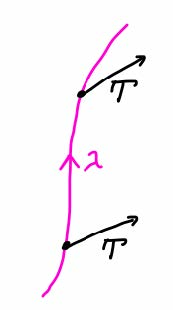
\includegraphics[width=2cm]{../img/parallel-transport.jpg}
\end{figure}
\noindent
In particular, a vector field $V^\mu(\lambda)$ supported on a curve $\gamma:\,\lambda\mapsto X^\mu$, is \textbf{parallel-transported} along the curve iff it is covariantly constant along $\gamma$
\begin{equation}\label{eqn:parallel-transport}\boxed{
\cder{V^\mu}{\lambda}=\der{V^\mu(\lambda)}{ \lambda}+\dot X^\rho(\lambda)\chris\mu\sigma\rho(X(\lambda))V^\sigma(\lambda)=0
}\end{equation}
This is a first order equation that can be always be integrated, then given $V^\mu(\lambda_0)$ one can define the corresponding parallel transported vector field uniquely through eq.~\eqref{eqn:parallel-transport}. 

If the connection is compatible with the metric (for instance if it is Levi-Civita connection) the parallel transport preserves the scalar product between vectors: if
\[\cder{V^\mu(\lambda)}{\lambda}=\cder{W^\mu(\lambda)}{\lambda}=0\]
then
\[\der{}{\lambda}(V^\mu W_\mu)=\cder {}{\lambda}(g_{\mu\nu}V^\mu W^\nu)=\cder{g_{\mu\nu}}{\lambda}V^\mu W^\nu+g_{\mu\nu}\p{\cder{V^\mu}{\lambda}W^\nu+V^\mu\cder{W^\nu}{\lambda}}=0\]
i.e. $V^\mu W_\mu$ is constant along the curve if $V^\mu$ and $W^\mu$ are parallel transported along $\gamma$. 

\begin{figure}[H]
\centering
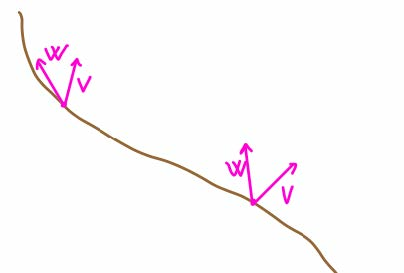
\includegraphics[width=5cm]{../img/parallel-transport-scalar-prod.jpg}
\end{figure}

In a flat space a straight line is a path that parallel-transports its own tangent vector. We can generalize this concept for more general connection introducing a new object. In particular \textbf{geodesic} are curves that satisfies following relation, namely \textbf{geodesics equation}:
\begin{equation}\label{eqn:geodesic-equation}\boxed{
\cder{\dot X(\lambda)}\lambda=\frac{\de^2 X^\mu}{\de\lambda^2}+\chris\mu\nu\rho(X)\der{X^\mu}\lambda\der{X^\nu}\lambda=0
}\end{equation}

\begin{figure}[H]
\centering
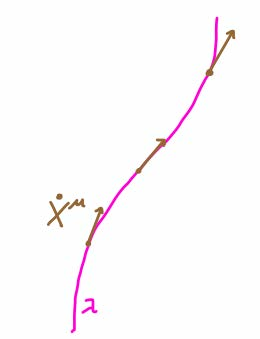
\includegraphics[width=4cm]{../img/geodesic.jpg}
\end{figure}

\noindent
Such curves can be thought heuristically as straightest possible curve in a curved space, and are exactly the particle's EoM for the affine parameter $\lambda$. This makes further manifest the invariance of the particle's EoM, indeed trajectories are a geometrical object independent from bulk coordinate since covariant derivative of a vector is a tensor. Moreover, in the case of LC connection a time-like geodesic can be equivalently characterized  as the curve between two fixed events that extremizes the proper time. 

Another important point is that using the compatibility between parallel transport and scalar product we can conclude that under parallel transport
\[\dot X^\mu(\lambda)\dot X_\mu(\lambda)=g_{\mu\nu}(X(\lambda))\dot X^\mu(\lambda)\dot X^\nu(\lambda)=\,\text{constant}\]
and then
\[\boxed{
\dot X^\mu(\lambda_0)\,\text{is time-like/space-like/null}\quad\Rightarrow\quad\dot X^\mu(\lambda)\,\text{is time-like/space-like/null }\,\forall \lambda
}\]
This means that we can distinguish between time-like, space-like and null geodesics. In particular, for massless particles we do no need to separately solve for $\dot X^2(\lambda)=0$, but it is sufficient to impose it at $\lambda=\lambda_0$. 

For space-like curves $X^\mu(\lambda)$, that is such that $g_{\mu\nu}(X)\dot X^\mu\dot X^\nu>0$, one can define the \textbf{proper length}
\[\Delta l=\int\de\lambda\,\sqrt{g_{\mu\nu}(X)\dot X^\mu\dot X^\nu}\]
and by following the same steps as for the particle's action, one can show that $\Delta s$ between two fixed points is extremized if the geodesic equation is satisfied, with Levi-Civita connection $\chris\mu\nu\rho$ and affine parameter in the form 
\[\lambda=al+b\]
for some constant $a$ and $b$ (geodesic equation does not change under this reparametrization). In particular (locally) shortest curves between two points are space-like geodesics. 

\begin{figure}[H]
\centering
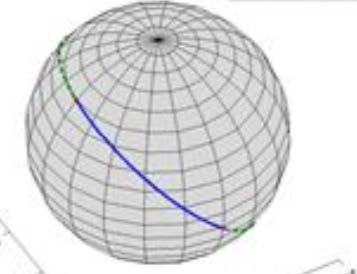
\includegraphics[width=5cm]{../img/extremized-geodesic.jpg}
\end{figure}

We said that geodesics parametrized by the affine parameter $\lambda$ coincides with EoM of point-particles. However, we may want to use a more general parameter $\sigma$ to describe the geodesics. Then the corresponding equation obtained from geodesic equation through a change of parameter is
\begin{equation}\label{geodesic-eqn-change-coord}\boxed{
\cder {\dot X^\mu(\sigma)}\sigma=\frac{\de^2 X^\mu}{\de\sigma^2}+\chris\mu\nu\rho\der{X^\nu}\sigma\der{X^\rho}{\sigma}=f(\sigma)\der{X^\mu}\sigma
}\end{equation}
with $f(\sigma)=-\p{\der\sigma\lambda}^{-2}\frac{\de^2\sigma}{\de\lambda^2}$ (prove this as an exercize). Viceversa, if this equation holds, then we can always fine an affine parameter $\lambda$ such that $f(\sigma)\der{X^\mu}\sigma=0$. 
Then, the condition eq.~\eqref{geodesic-eqn-change-coord} requires that $\dot X^\mu$ is parallely transported along $\gamma$, up to possible rescaling of its length. This gives a more general description of geodesics respect to eq.~\eqref{eqn:geodesic-equation}, indeed eq.~\eqref{geodesic-eqn-change-coord} states that a geodesics is a curve such that the covariant derivative of the tangent vector is proportional to the tangent vector itself (previous definition states that tangent vector must be covariantly constant). 

One may consider more general time-like trajectories parametrized by proper time and define \textbf{four-velocity} as
\[u^\mu=\der{X^\mu}{\tau}\]
Then using the notion of covariant derivative for a trajectory, define \textbf{four-acceleration} as
\[\alpha^\mu=\cder{u^\mu}\tau=\frac{\de^2 X^\mu}{\de\tau^2}+\chris\mu\rho\sigma\der{X^\rho}\tau\der{X^\sigma}{\tau}\]
With the definition, as expected, geodesic condition is equivalent to 
\[\alpha^\mu=0\]
i.e. the 4-velocity is covariantly constant. This equation also define the EoM for free particles in a curved space. Whenever a force (not the gravitational one) is applied to a particle, the effect of this forces can be codified in a \textbf{four-force} defined as
\[f^\mu=m\alpha^\mu=m\cder{u^\mu}\tau\]
As in the special relativistic case, 4-velocity and 4-acceleration satisfies useful properties. First of all
\[u^\mu u_\mu=-1\]
Then, by applying the covariant derivative on both sides of this equation and using the  metricity of the connection, we obtain
\[u_\mu\alpha^\mu=g_{\mu\nu}u^\mu\alpha^\nu=0\]
and this means that $\alpha^\mu$ is space-like. 
Finally, we can define \textbf{proper acceleration} as the acceleration in the proper instance frame of the particle itself
\[\alpha=\sqrt{\alpha^\mu\alpha_\mu}\]









\end{document}